\documentclass{slide}

\usepackage[T1]{fontenc}  % Suddenly required to compile using GH Actions.
\usepackage{tikz}
\usetikzlibrary{snakes}
\usetikzlibrary{intersections}
\usetikzlibrary{shapes.geometric}

\usepackage{languages}

\title{Infrastructure as Code}
\subtitle{Software Architecture}
\author{Brae Webb \& Richard Thomas}
\date{\week{4}}


\begin{document}

\maketitle
\note[itemize]{
    \item Do a quick poll.
    \item Who has heard the term IaC before this course?
    \item Who has used IaC before this course?
}

\point[Infrastructure as Code]{How did we get here?}

\point[Pre-2000]{The \highlight{Iron Age}}

\point[\Large Iron Age]{
\begin{center}
\only<1>{
\includegraphics[width=0.25\textwidth]{diagrams/iron-age}
}
\only<2>{
\includegraphics[width=0.25\textwidth]{diagrams/iron-age-names}
}
\end{center}
}
\note{Developer only had a few machines --- so few the machines often got fun names.}

\point[\Large Scaling]{
\begin{center}
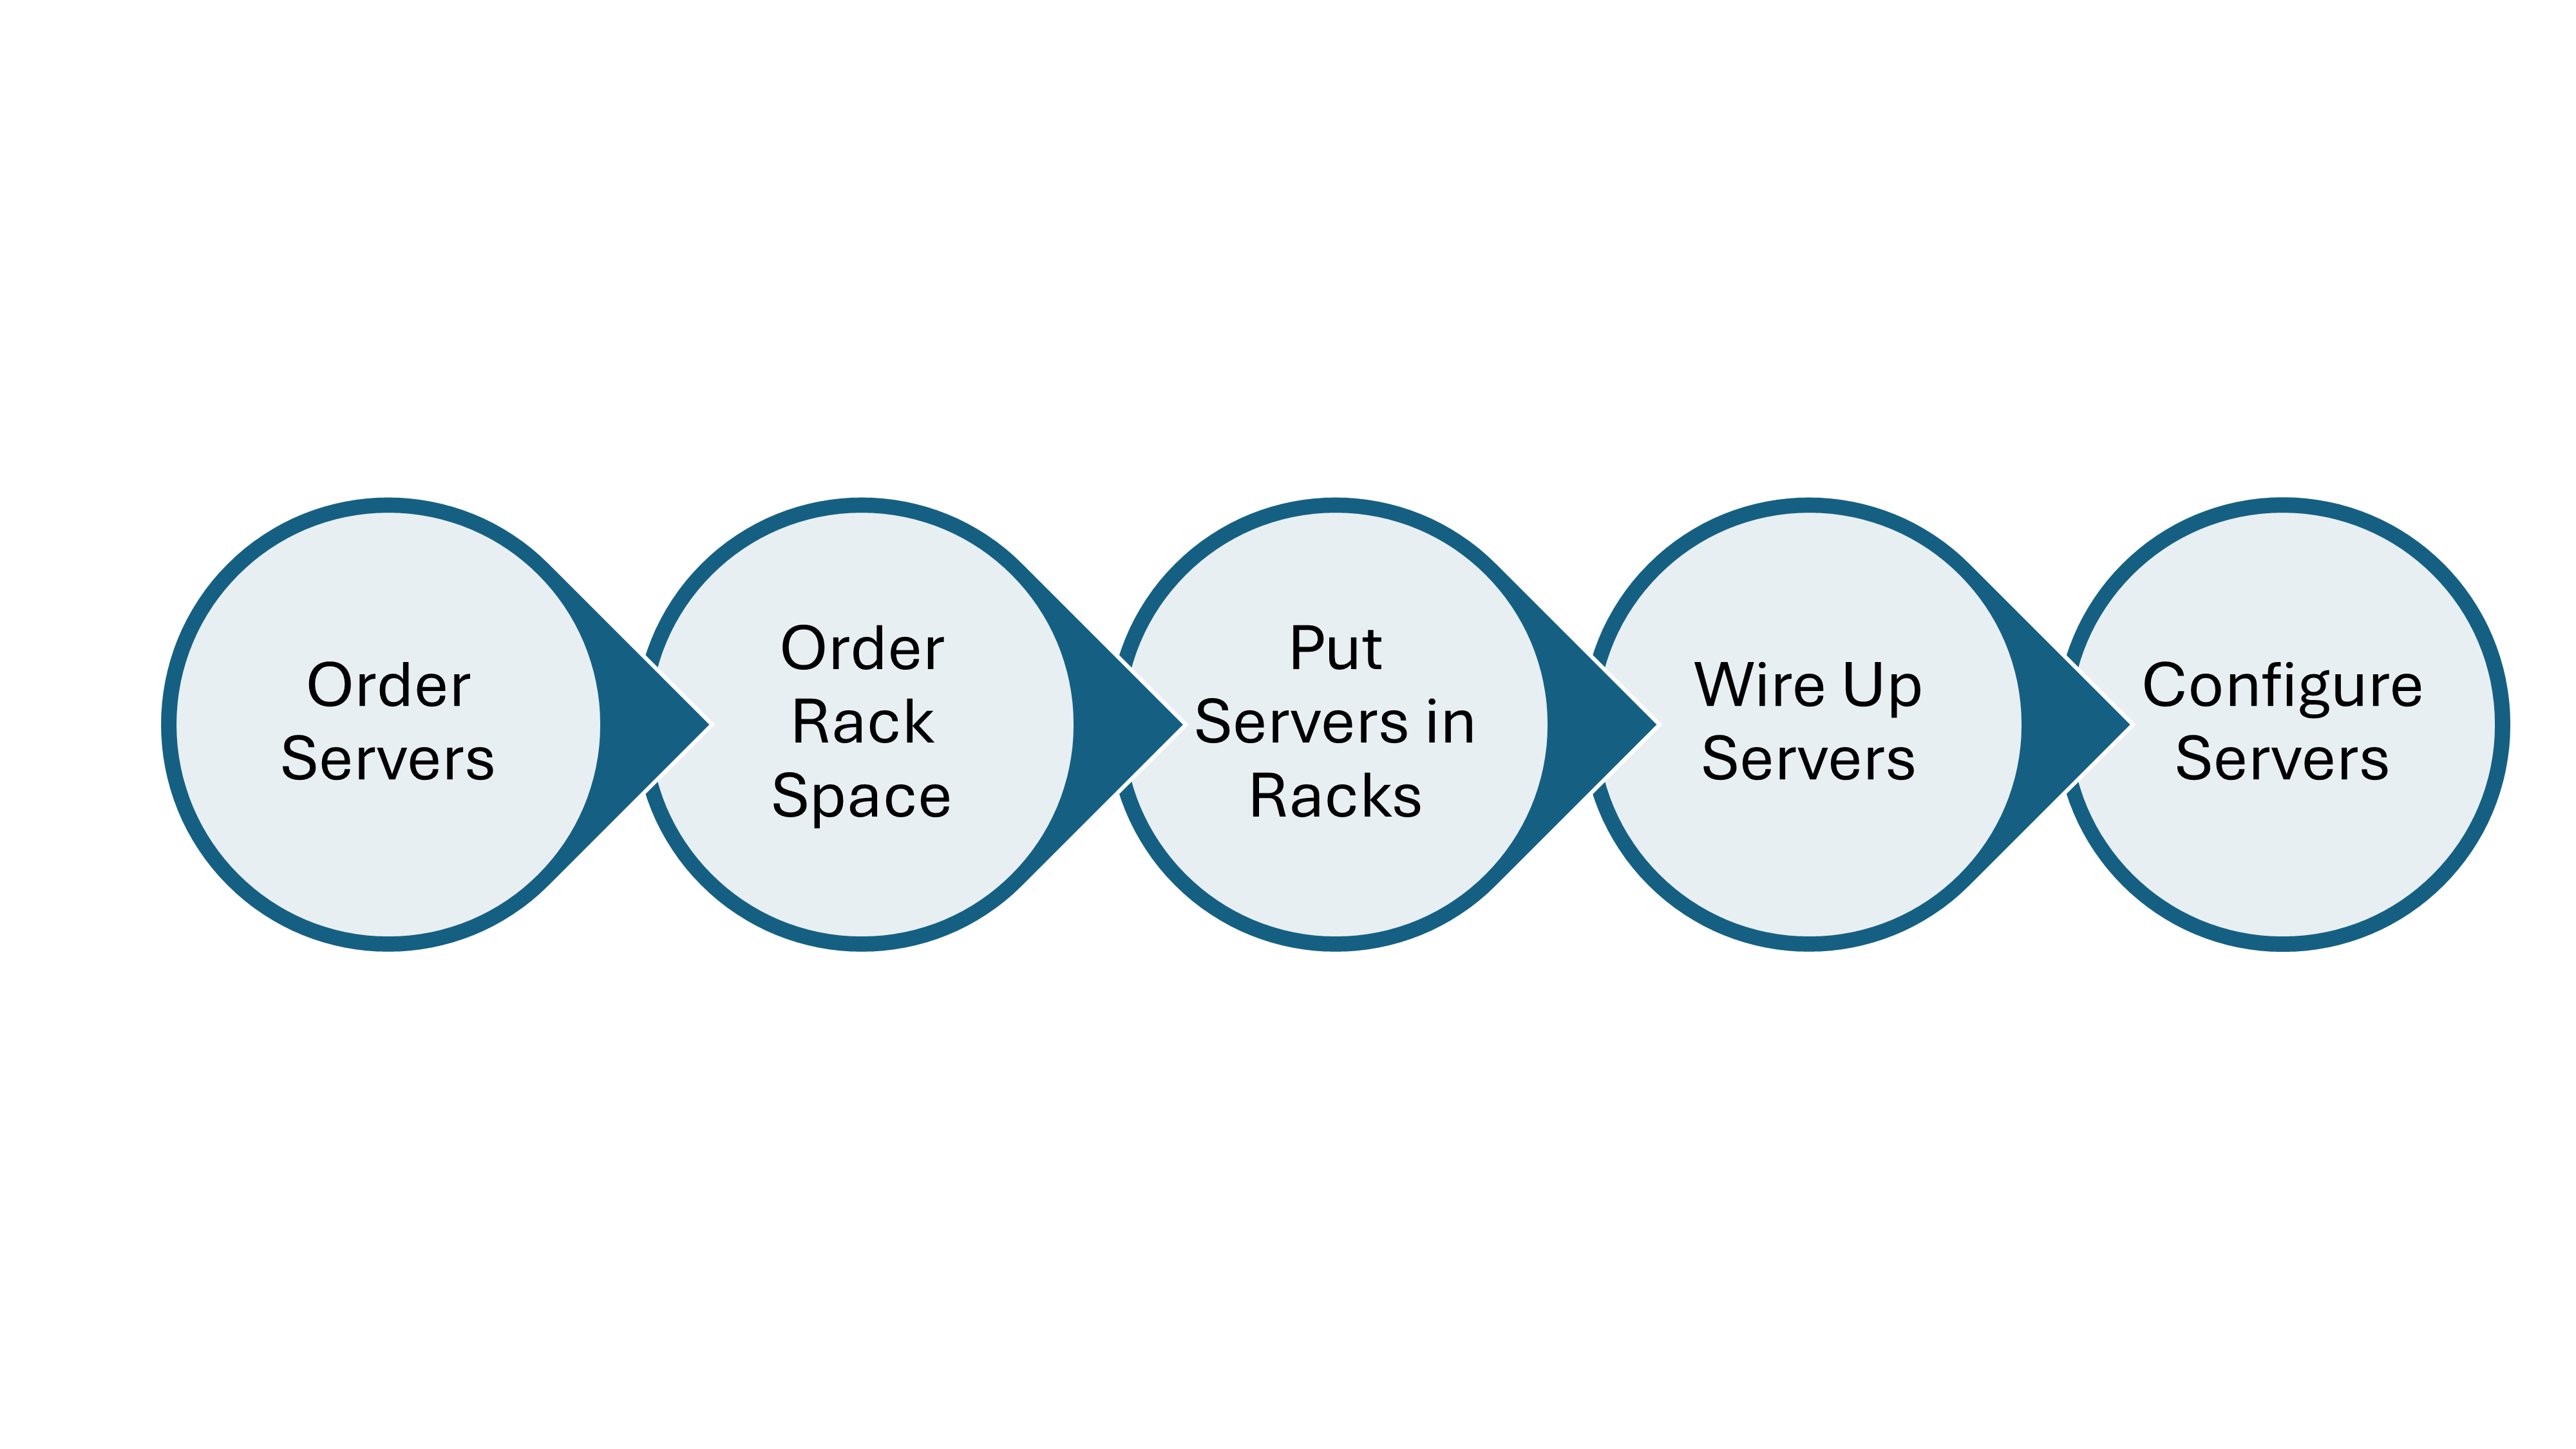
\includegraphics[trim=50 75 20 75,clip,width=0.95\textwidth]{diagrams/physical_server_deployment}
\end{center}
}
\note{
I used to have scheduling examples for software projects,
where ordering servers was on the critical path, and had to happen before software development started.
}

\point[Introducing...]{The \highlight{Cloud Age}}

\point[\Large The Cloud Age]{
\begin{center}
\includegraphics[width=0.5\textwidth]{diagrams/cloud-age}
\end{center}
}
\note[itemize]{
    \item Summarise: things got complicated quickly, we need more hardware and it's easier to provision.
    \item Largely thanks to virtualisation --- no physical activity for a new machine.
}

\point[When faced with complexity]{Automate it!}
\note[itemize]{
    \item We have too much to manage to do it manually.
    \item We're about to start enumerating automation techniques.
}

\begin{frame}{The larger story}

\begin{description}[<+->][leftmargin=!,labelwidth=\widthof{Data}]
    \item[Server Config] Config Management
    \item[Application Config] Config Files
    \item[Provisioning] Infrastructure Code
    \item[Building] Continuous Integration
    \item[Deployment] Continuous Deployment
    \item[Testing] Automated Tests
    \item[Database Administration] Schema Migration
    \item[Specifications] Behaviour Driven Development
\end{description}

\end{frame}

\begin{frame}
\large
\only<1->{
\begin{defn}[Infrastructure Code]
    Code that provisions and manages \highlight{infrastructure resources}.
\end{defn}}

\only<2->{
\begin{defn}[Infrastructure Resources]
    Compute resources, networking resources, and storage resources.
\end{defn}}
\end{frame}

\point[\Large Infrastructure Code]%
{   
\begin{center}\Large
    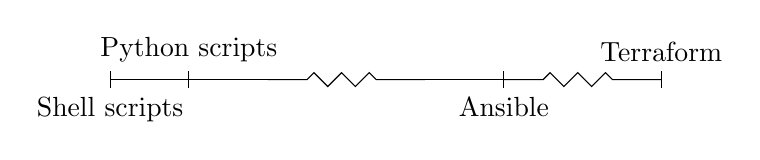
\begin{tikzpicture}[
        snake=zigzag,line before snake=5mm,line after snake=5mm
      ]
      \draw (0,0) -- (2,0);
      \draw[snake] (2,0) -- (4,0);
      \draw (4,0) -- (5,0);
      \draw[snake] (5,0) -- (7,0);
  
      \foreach \x in {0,1,5,7} \draw (\x cm,3pt) -- (\x cm,-3pt);
  
       \draw (0,0) node[below=3pt] {Shell scripts} node[above=3pt] {};
       \draw (1,0) node[below=3pt] {} node[above=3pt] {Python scripts};
       \draw (3,0) node[below=3pt] {} node[above=3pt] {};
       \draw (4,0) node[below=3pt] {} node[above=3pt] {};
       \draw (5,0) node[below=3pt] {Ansible} node[above=3pt] {};
       \draw (6,0) node[below=3pt] {} node[above=3pt] {};
       \draw (7,0) node[below=3pt] {} node[above=3pt] {Terraform};
    \end{tikzpicture}
\end{center}
}
\note{IC often thought of as the right-hand side but includes all.}

\begin{frame}[fragile]{Shell Scripts}
\begin{code}[language=bash]{}
#!/bin/bash

SG=$(aws ec2 create-security-group ...)

aws ec2 authorize-security-group-ingress --group-id "$SG"

INST=$(aws ec2 run-instances --security-group-ids "$SG" \
         --instance-type t2.micro)
\end{code}
\end{frame}
\note{Using AWS CLI to create EC2 access like the practical.}

\begin{frame}[fragile]{Python}
\begin{code}[language=python]{}
import boto3

def create_instance():
    ec2_client = boto3.client("ec2", region_name="us-east-1")
    response = ec2.create_security_group(...)
    security_group_id = response['GroupId']

    data = ec2.authorize_security_group_ingress(...)

    instance = ec2_client.run_instances(
        SecurityGroups=[security_group_id],
        InstanceType="t2.micro",
        ...
    )
\end{code}
\end{frame}
\note{Using AWS Python library (boto3).}


\begin{frame}[fragile]{Terraform}
\begin{code}[language=terraform]{}
resource "aws_instance" "hextris-server" {
    instance_type = "t2.micro"
    security_groups = [aws_security_group.hextris-server.name]
    ...
}

resource "aws_security_group" "hextris-server" {
    ingress {
        from_port = 80
        to_port = 80
        ...
    }
    ...
}
\end{code}
\end{frame}
\note{Finally, Terraform.}

\question{Notice anything different?}
\note[itemize]{
    \item Prompting for declarative.
    \item Might notice verbosity.
}

\point[\Large The \highlight{main} difference]{Imperative vs. Declarative}
\note[itemize]{
    \item \highlight{Imperative} -- Describe the steps to take to deploy the infrastructure
    \item \highlight{Declarative} -- Describe the desired infrastructure
    \item IC is heading towards a more \highlight{declarative} paradigm.
}

\point[\LARGE Declarative IaC]
{
    \vspace{1em}
    \begin{itemize}
        \item Define your \highlight{desired} infrastructure state
        \begin{itemize}
            \item\LARGE as code
        \end{itemize}
        \vspace{0.5em}
        \item Engine interprets difference between the \highlight{desired} and \highlight{actual} state
        \begin{itemize}
            \item\LARGE Modifying infrastructure to deliver \highlight{desired} state
        \end{itemize}
    \end{itemize}
}

\point[\Large Infrastructure Code]{
\Large
\begin{itemize}[<+->]
    \item Provisions and manages \highlight{infrastructure resources}.
    \item Only one part of the movement to \highlight{automate} the complexities of development.
    \item Ranges from simple shell scripts up to\dots?
    \item Tendency to be \highlight{declarative}.
\end{itemize}
}
\note{Summarising what we've already covered.}

\point[\Large Typo?]{Infrastructure Code $\neq$ Infrastructure \highlight{as} Code}
\note[itemize]{
    \item Mention that this distinction is ours.
    \item Real world unfortunately mixes the two.
}

\definition{Infrastructure as Code}%
{Following the same \highlight{good coding practices} to manage Infrastructure Code as standard code.}

\point[\Large Warning!]{Infrastructure as Code still \highlight{early} and quite \highlight{bad}.}
\note[itemize]{
    \item Code reuse is low.
    \item Importing existing resources is non-trivial.
    \item Refactoring is painful.
    \item State management can be tricky.
}

\question{What are \highlight{good coding practices}?}
\note{Ask the class.}

\point[\Large Good Coding Practice \#1]{\highlight{Everything} as Code}
\note{A practice we do but barely discuss in `regular' programming because it doesn't make sense not to do it.}

\begin{frame}[fragile]
\begin{code}[language=shell]{}
#!/bin/bash

./download-dependencies
./build-resources
cp -r output/* artifacts/
\end{code}

\only<2>{\bash{cp: directory artifacts does not exist}}
\end{frame}
\note{An example of relying on external state in `regular' programming.}

\begin{frame}[fragile]
\begin{code}[language=terraform]{}
resource "aws_instance" "hextris-server" {
    instance_type = "t2.micro"
    security_groups = ["sg-6400"]
    ...
}
\end{code}
\end{frame}
\note{Draw a parallel to the bash example and this, which relies on `sg-6400' existing.}

\begin{frame}[fragile]
\begin{code}[language=terraform]{}
resource "aws_instance" "hextris-server" {
    instance_type = "t2.micro"
    security_groups = [aws_security_group.hextris-server.name]
    ...
}

resource "aws_security_group" "hextris-server" {
    ingress {
        from_port = 80
        to_port = 80
        ...
    }
    ...
}
\end{code}
\end{frame}
\note{The better approach.}

\point[\Large Everything as code avoids]{
Configuration drift
}

\point[\Large Configuration drift creates]{
Snowflakes
}
\note[itemize]{
    \item Snowflakes: magical machines that `just work' and everyone is afraid to touch.
    \item Snowflake because they're unique and easy to break, because no one knows how it works.
}

\point[\Large Benefits]{
\begin{enumerate}
    \item Reproducible
\end{enumerate}
}

\point[\Large Good Coding Practice \#2]{Version Control}

\point[\Large Benefits]{
\begin{enumerate}
    \item Restorable
    \item Accountable
\end{enumerate}
}

\point[\Large Good Coding Practice \#3]{Automation}

\point[\Large Benefits]{
\begin{enumerate}
    \item Consistent
\end{enumerate}
}
\note{Automatically applying or checking IC is in sync means the main branch is consistent with reality.}

\point[\Large Good Coding Practice \#4]{Code Reuse}

\point[\Large Benefits]{
\begin{enumerate}
    \item Better\footnote{generally} code
    \item Less work
    \item Only one place to update (or verify)
\end{enumerate}
}

\point[\Large Good Coding Practice \#5]{Testing}

\begin{frame}{Test Pyramid}
    \begin{center}
    \begin{tikzpicture}
    \coordinate (A) at (-5,0) {};
    \coordinate (B) at ( 5,0) {};
    \coordinate (C) at (0,7) {};
    \draw[name path=AC] (A) -- (C);
    \draw[name path=BC] (B) -- (C);
    \foreach \y/\A in {0/Unit Testing,2/Integration Testing,4/End-to-end Testing} {
        \path[name path=horiz] (A|-0,\y) -- (B|-0,\y);
        \draw[name intersections={of=AC and horiz,by=P},
                name intersections={of=BC and horiz,by=Q}] (P) -- (Q)
            node[midway,above] {\A};
    }
    \end{tikzpicture}
    \end{center}
\end{frame}
\note[itemize]{
    \item Traditional test pyramid.
    \item Unit testing relies on isolated testing.
    \item But\dots isolated testing doesn't make \highlight{much} sense for IaC.
}

\begin{frame}{IaC Test Pyramid}
    \begin{center}
    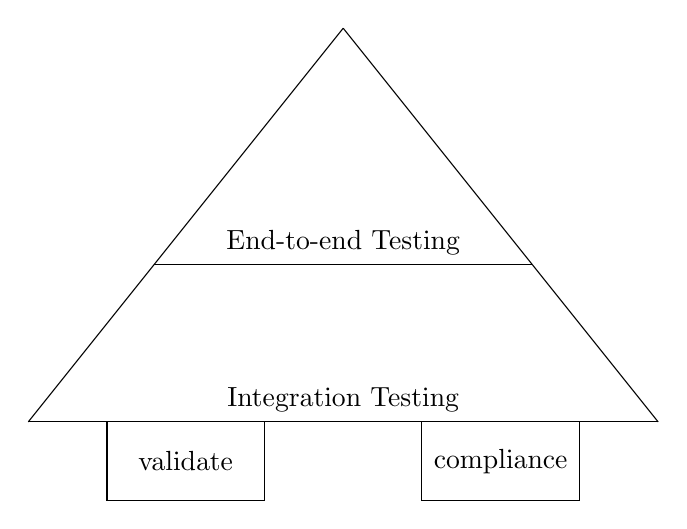
\begin{tikzpicture}
    \coordinate (A) at (-4,2) {};
    \coordinate (B) at ( 4,2) {};
    \coordinate (C) at (0,7) {};
    \draw[name path=AC] (A) -- (C);
    \draw[name path=BC] (B) -- (C);
    \foreach \y/\A in {2/Integration Testing,4/End-to-end Testing} {
        \path[name path=horiz] (A|-0,\y) -- (B|-0,\y);
        \draw[name intersections={of=AC and horiz,by=P},
                name intersections={of=BC and horiz,by=Q}] (P) -- (Q)
            node[midway,above] {\A};
    }
    \node at (-2,1.5) [rectangle,draw,minimum height = 1cm,,minimum width = 2cm] (validate) {validate};
    \node at (2,1.5) [rectangle,draw,minimum height = 1cm,,minimum width = 2cm] (compliance) {compliance};
    \end{tikzpicture}
    \end{center}
\end{frame}

\begin{frame}[fragile]
\begin{code}[language=go]{}
func TestTerraformAwsInstance(t *testing.T) {
    terraformOptions := terraform.WithDefault(t, &terraform.Options{
        TerraformDir: "../week03/",
    })

    defer terraform.Destroy(t, terraformOptions)
    terraform.InitAndApply(t, terraformOptions)

    publicIp := terraform.Output(t, terraformOptions, "public_ip")
    url := fmt.Sprintf("http://%s:8080", publicIp)

    http_helper.HttpGetWithCustomValidation(t, url, nil, 200, 
        func(code, resp) { code == 200 &&
                             strings.Contains(resp, "hextris")})
}
\end{code}
\end{frame}
\note{An example of validation.}

\begin{frame}[fragile]
\begin{code}[language=Gherkin]{}
Feature: Define AWS Security Groups

Scenario: Only selected ports should be publicly open
    Given I have AWS Security Group defined
    When it contains ingress
    Then it must only have tcp protocol and port 22,443 for 0.0.0.0/0
\end{code}
\end{frame}
\note{An example of compliance testing.}

\point[\Large Benefits]{
\begin{enumerate}
    \item Trust
\end{enumerate}
}

\point[\Large Prac Next Week]{Learn how to use Terraform to write IaC and deploy resources on AWS.}

\end{document}